\documentclass[10pt]{article}

% This report is intended to compile on a standard TeX Live or Overleaf
% installation together with the generated PNG figures in the project tree.
\usepackage[utf8]{inputenc}
\usepackage[T1]{fontenc}
\usepackage{lmodern}
\usepackage[letterpaper,margin=0.82in]{geometry}
\usepackage{microtype}
\usepackage{amsmath,amssymb}
\usepackage[table]{xcolor}
\usepackage{booktabs}
\usepackage{tabularx}
\usepackage{array}
\usepackage{multirow}
\usepackage{enumitem}
\usepackage{graphicx}
\graphicspath{{model_outputs_single_drone/figures/}{../model_outputs_single_drone/figures/}{outputs_single_drone/figures/}{../outputs_single_drone/figures/}}
\usepackage{caption}
\usepackage{subcaption}
\usepackage{float}
\usepackage{placeins}
\usepackage{hyperref}
\usepackage{url}
\usepackage{tikz}
\usepackage{pgfplots}
\usetikzlibrary{arrows.meta,positioning,shapes.geometric,fit}
\pgfplotsset{compat=1.18}

\definecolor{navy}{HTML}{17365D}
\definecolor{blue}{HTML}{2F5597}
\definecolor{lightblue}{HTML}{D9EAF7}
\definecolor{paleblue}{HTML}{EEF5FB}
\definecolor{lightgray}{HTML}{F2F2F2}
\definecolor{midgray}{HTML}{666666}
\definecolor{goodgreen}{HTML}{DDEBF7}
\definecolor{warnorange}{HTML}{FCE4D6}

\hypersetup{
  colorlinks=true,
  linkcolor=navy,
  citecolor=navy,
  urlcolor=blue,
  pdftitle={WEPAStacks Inbound Congestion Prediction and Single-Drone Routing},
  pdfsubject={Machine Learning Assignment 2 Project Report}
}

\setlength{\parindent}{0pt}
\setlength{\parskip}{0.55em}
\setlist[itemize]{leftmargin=1.45em,itemsep=0.25em,topsep=0.25em}
\setlist[enumerate]{leftmargin=1.65em,itemsep=0.25em,topsep=0.25em}
\captionsetup{font=small,labelfont=bf}
\renewcommand{\arraystretch}{1.18}
\newcolumntype{Y}{>{\raggedright\arraybackslash}X}
\newcolumntype{C}[1]{>{\centering\arraybackslash}p{#1}}
\newcommand{\code}[1]{\nolinkurl{#1}}
\newcommand{\R}{\mathbb{R}}

\title{\textbf{WEPAStacks Inbound Congestion Prediction and Single-Drone Routing}\\[0.45em]
\large An MLP-Filtered Ant Colony Optimisation Framework}
\author{Undergraduate Machine Learning Project Report}
\date{September 2026}

\begin{document}
\maketitle

\begin{abstract}
This project studies whether recent inbound activity can support warehouse-buffer congestion prediction and proactive pickup decisions. The provided WEPAStacks delivery records are aggregated into 15-minute intervals for four inbound points. A multilayer perceptron (MLP) maps seven current-and-past features to a sigmoid risk score for each warehouse. The simulated target is positive when the current stock plus arrivals during the next 60 minutes reaches 80\% of warehouse capacity under a no-drone counterfactual.

The updated routing design deliberately separates prediction from optimisation. Warehouses with goods are passed to ant colony optimisation (ACO) only when their MLP score is at least 0.70. ACO then uses pheromone and distance---not the MLP score---to construct one route for one simulated drone. Its objective first penalises unvisited active warehouses and then route distance. On the chronological test set, the MLP at the fixed 0.70 threshold records 98.59\% precision, 95.45\% recall, and 96.99\% F1, compared with 87.69\% F1 for a current-fill rule. This evidence is limited: all positive validation and test labels occur at Warehouse~1. The available routing output covers only 20 intervals and one ACO seed, so it is reported as a smoke test rather than evidence of operational superiority.
\end{abstract}

\textbf{Keywords:} warehouse congestion, multilayer perceptron, time-series classification, ant colony optimisation, drone routing, WEPAStacks

\tableofcontents
\newpage

\section{Introduction}

Inbound congestion occurs when arriving goods accumulate faster than a handling system can remove them. A useful decision-support system should distinguish current or near-term congestion from lower-risk states, and its pickup policy should respect distance, energy, and payload limits. This project investigates these linked but distinct tasks. The MLP estimates current-or-next-hour threshold risk. Its score is used once, as a filter. ACO receives only the warehouses that pass the filter and constructs a single-drone route from their current goods and distances.

The practical motivation is that a reactive fill rule uses only the present queue. It does not directly use recent arrival intensity, so it may activate later than a predictor that recognises a rising pattern. This motivates testing an MLP, but does not establish that machine learning is necessary. The prediction stage is therefore compared with both an always-negative rule and a current-fill rule. At the operational stage, MLP--ACO is compared with nearest-first, fullest-first, and ACO-current. The MLP is kept small because the input is tabular and its recent history is already summarised; its deployment suitability is not assumed.

The central research question is:

\begin{quote}
On the chronological held-out period, does filtering warehouses with an MLP risk threshold before single-drone ACO reduce overflow relative to current-fill routing, while respecting route-distance, energy, and payload constraints?
\end{quote}

The prediction stage asks whether seven present-and-past features improve threshold classification over simple rules. The operational stage asks whether the resulting filter improves routing outcomes. A high classification score alone cannot answer the operational question.

\section{Task Definition}

\subsection{Primary contribution and project boundary}

The proposed contribution is an MLP-filtered ACO pipeline for one drone. The MLP produces one score per warehouse. A hard threshold of 0.70 determines which non-empty warehouses are visible to ACO. The score is not reused as an urgency weight, projected-stock estimate, or ACO objective term. This separation makes the role of machine learning testable: it changes the candidate set, while ACO remains a distance-based route optimiser.

The report uses a drone-only queue definition. Goods leave a simulated warehouse only when the single drone collects them. Battery is restored at the beginning of every 15-minute interval, representing replacement or charging at the depot. The earlier service-rate and multi-drone designs are outside the scope of the current experiment. The training-state simulator and deployment simulator use the same warehouse capacities, single-drone configuration, per-interval battery policy, and queue-update equations.

\subsection{Scope and distinction between provided and simulated data}

The project distinguishes fields in the provided WEPAStacks records from experimental assumptions introduced by the simulation. The supplied fields describe a temporal stream of inbound events; the current file does not include four geographically separated warehouses, drone specifications, a central depot, or measured congestion labels.

\begin{table}[H]
\centering
\caption{Provided dataset information and simulated assumptions}
\label{tab:real-simulated}
\small
\begin{tabularx}{\textwidth}{>{\bfseries}p{0.20\textwidth}YY}
\toprule
Category & Used in the project & Interpretation \\
\midrule
Provided WEPAStacks fields & Arrival time, inbound dock, SKU, batch, and week where available & The event records determine time-varying arrival demand in the experiment. The baseline model uses arrival time and dock; SKU and batch are excluded. \\
Simulated system state & Queue length, historical drone pickups, warehouse capacities, and congestion at 80\% capacity & These variables define a synthetic prediction target. They are not observed ground truth, and reproducibility must be confirmed from the final configuration and seed records. \\
Simulated routing environment & Four satellite warehouses, planar coordinates, central depot, and one drone with payload, battery, energy, and route-distance limits & These values define the proposed routing experiment. One event is treated as one standardised cargo unit, not as a claim that a small drone carries a physical pallet. \\
\bottomrule
\end{tabularx}
\end{table}

\subsection{Training interface}

Each training observation represents one dock at the end of a 15-minute interval. The input vector is
\begin{equation}
\mathbf{x}_{i,t} = [r_{i,t},\; a_{i,t},\; \bar{a}^{(60)}_{i,t},\; d_{i,1},\; d_{i,2},\; d_{i,3},\; d_{i,4}] \in \R^7,
\end{equation}
where $r_{i,t}$ is the buffer fill ratio, $a_{i,t}$ is the current number of arrivals, $\bar{a}^{(60)}_{i,t}$ is the mean arrival count over the current and previous three intervals, and $d_{i,j}$ is a one-hot dock indicator. The feature definition is intended to restrict input values to information available at or before time $t$; this property must be confirmed in the final leakage audit.

The binary training target assumes that no drone will collect goods during the next four intervals. It is
\begin{equation}
y_{i,t}=\mathbb{1}\!\left[\max_{h\in\{1,2,3,4\}}
\left(A_{i,t}+\sum_{s=1}^{h}a_{i,t+s}\right) \geq 0.8K_i\right],
\label{eq:target}
\end{equation}
where $A_{i,t}$ is the available stock before the current pickup decision and $K_i$ is warehouse capacity. The configured capacities are 200 units for Warehouse~1 and 80 units for Warehouses~2--4. Future arrivals are required for historical label construction. The feature-building procedure is intended to exclude them from the input vector, and that separation must be verified before final reporting.

\begin{table}[H]
\centering
\caption{Technical input and output specification}
\label{tab:io}
\small
\begin{tabularx}{\textwidth}{p{0.15\textwidth}p{0.20\textwidth}YY}
\toprule
Phase & Interface & Valid input & Output \\
\midrule
Training & One warehouse--interval sample & A seven-value vector in the fixed order shown above; the three numeric features are scaled from training statistics and the four dock indicators remain binary & One binary label indicating whether no-drone stock reaches 80\% capacity during the next four intervals \\
MLP deployment & One simultaneous four-warehouse state & A $4\times7$ \texttt{float32} feature matrix containing current fill ratio, current arrivals, trailing four-interval mean, and dock identity & A vector $\hat{\mathbf p}_t\in[0,1]^4$ containing one sigmoid score per warehouse; scores are not assumed to be calibrated probabilities \\
Pre-ACO filter & Current goods and four MLP scores & Warehouse $i$ is retained only if $A_{i,t}>0$ and $\hat p_{i,t}\geq0.70$ & A sorted mapping from active warehouse identifier to currently available goods \\
ACO deployment & Filtered goods, a $5\times5$ distance matrix, one drone state, ACO parameters, and seed & Non-negative goods; valid depot/warehouse nodes; positive payload, energy, battery, and maximum-distance limits & One depot-to-depot route, proportional pickup amounts, route distance, energy used, remaining active goods, objective value, and validation status \\
\bottomrule
\end{tabularx}
\end{table}

\subsection{Expected behaviour}

Given a low fill ratio and low recent arrivals, the MLP should produce a lower score than for a state close to the congestion boundary with sustained arrivals. Because the target includes stock that is already at the 80\% threshold, evaluation must distinguish current-state detection from genuine below-threshold forecasting. At deployment, a score of 0.70 is included and 0.699 is excluded. A warehouse with no goods is excluded even if its score is high. ACO may visit only retained warehouses. The route must start and end at depot 0, visit a warehouse at most once, remain within 30~km and 30 energy units, and collect at most 30 cargo units.

Two thresholds have different meanings. The congestion threshold of 0.80 defines the simulated target in terms of capacity. The operational score threshold of 0.70 filters warehouses before routing and is fixed in the current specification. A validation-optimal threshold is saved only as a diagnostic; it does not control the route. This distinction prevents the reported validation threshold from silently changing the operational experiment.

\subsection{Evaluation questions and success criteria}

\begin{table}[H]
\centering
\caption{Questions and pre-declared evidence required to answer them}
\label{tab:success-criteria}
\small
\begin{tabularx}{\textwidth}{p{0.16\textwidth}YY}
\toprule
Question & Evidence & Success criterion \\
\midrule
Prediction & PR--AUC, ROC--AUC, precision, recall, F1, confusion matrix, and per-warehouse support on chronological validation and test data & Compare with always-negative and current-fill baselines; do not generalise positive-class performance to a warehouse without positive support. \\
Primary routing & Overflow, collected units, energy, distance, sorties, active-warehouse visits, runtime, and independently recomputed constraint checks & Compare MLP--ACO with nearest-first, fullest-first, and ACO-current on identical held-out arrivals. \\
Stability & Repeated ACO runs on identical states and arrival streams & Use the ten configured seeds for stochastic policies and report mean and standard deviation; label any shorter run as diagnostic. \\
\bottomrule
\end{tabularx}
\end{table}

\section{Dataset and Preprocessing}

\subsection{Dataset structure and quality}

The supplied WEPAStacks documentation describes 89 days of operations in a finished-goods warehouse and three source files: a layout file, an order-event file, and an initial-fill file. The current implementation does not consume all three files directly. It uses a cleaned CSV derived from delivery events at inbound points 1--4; retrieval events, outbound points, the original layout, and initial inventory are outside the present learning interface.

The current cleaned dataset contains 205,258 inbound events and nine fields: arrival time, relative day, hour, minute, 15-minute time bin, dock, SKU, batch, and week. It covers relative days 2--89. Preliminary checks recorded by the current preprocessing workflow did not identify missing values, invalid dock identifiers, negative arrival times, or fully duplicated rows. The workflow also reported agreement between the derived day, hour, minute, and time-bin fields and arrival time. These checks should be rerun and independently reviewed before submission. There are 4,763 repeated arrival-time and dock combinations; they are currently retained because multiple distinct cargo events may occur at the same dock in the same second.

An evident data-quality concern is representativeness. Dock~1 contains 93.26\% of all events, while Docks~2--4 disappear early in the timeline. In the current cleaned file, events after day~39 are assigned only to Dock~1. The reason for this pattern is not established by the dataset and should not be inferred without additional metadata.

\begin{figure}[H]
\centering
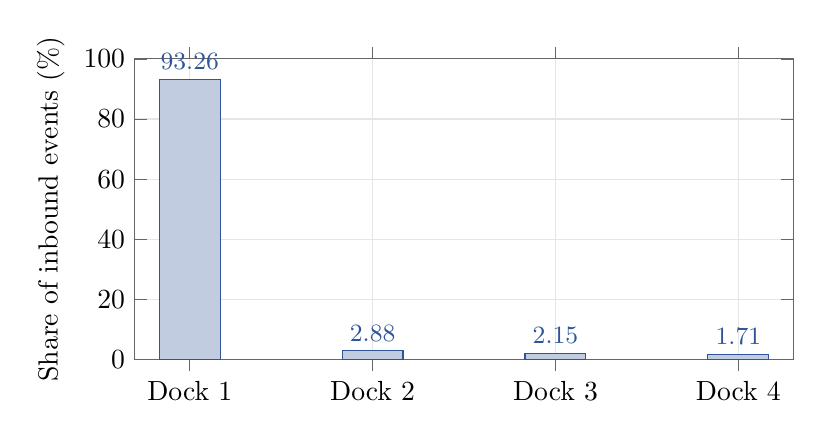
\begin{tikzpicture}
\begin{axis}[
  width=0.82\textwidth,
  height=5.4cm,
  ybar,
  bar width=22pt,
  ymin=0,ymax=100,
  ylabel={Share of inbound events (\%)},
  symbolic x coords={Dock 1,Dock 2,Dock 3,Dock 4},
  xtick=data,
  nodes near coords,
  nodes near coords align={vertical},
  every node near coord/.append style={font=\small},
  grid=major,
  grid style={draw=gray!20},
  axis line style={draw=midgray},
  tick style={draw=midgray},
  fill=blue!75,
]
\addplot coordinates {(Dock 1,93.26) (Dock 2,2.88) (Dock 3,2.15) (Dock 4,1.71)};
\end{axis}
\end{tikzpicture}
\caption{Inbound-event distribution by dock. Class weights may compensate for label imbalance, but they do not resolve unequal dock coverage.}
\label{fig:dock-distribution}
\end{figure}

\begin{table}[H]
\centering
\caption{Temporal coverage and arrival distribution by dock}
\label{tab:dock-coverage}
\small
\begin{tabular}{lrrrrrr}
\toprule
Dock & Events & Share & First day & Last day & Active days & Zero intervals \\
\midrule
1 & 191,428 & 93.26\% & 2 & 89 & 88 & 20.25\% \\
2 & 5,902 & 2.88\% & 2 & 39 & 12 & 92.65\% \\
3 & 4,421 & 2.15\% & 2 & 18 & 8 & 94.78\% \\
4 & 3,507 & 1.71\% & 2 & 11 & 5 & 95.83\% \\
\bottomrule
\end{tabular}
\end{table}

\subsection{Aggregation and zero intervals}

Arrival time is divided by 900 seconds and rounded down to obtain a 15-minute time bin. Events are grouped by time bin and dock. A complete Cartesian grid is then created from all 8,395 consecutive time bins and the four docks, producing 33,580 dock--interval rows before rolling and future-horizon exclusions. Missing counts are filled with zero. This step is necessary because a missing event row may mean that an active dock received no goods during the interval.

The same operation also creates a limitation. For Docks~2--4, a zero after the final recorded event may mean either zero demand or missing/inactive coverage. The dataset has no \texttt{dock\_active} field, so the pipeline cannot distinguish these cases. The report therefore treats late zero rows for Docks~2--4 cautiously.

\subsection{Rolling features, queue simulation, and leakage control}

The 60-minute rolling feature is the mean of arrivals in the current and previous three intervals. The first three rows for each dock are discarded because a complete window is unavailable. Historical training states are generated chronologically by a fixed fullest-first drone policy. The policy is designed to read current available goods, current battery, capacities, and distances without using future arrivals or MLP predictions. This restriction remains part of the final leakage audit. The state update is
\begin{align}
A_{i,t} &= Q_{i,t}+a_{i,t},\\
R_{i,t} &= \max(0,A_{i,t}-P_{i,t}),\\
O_{i,t} &= \max(0,R_{i,t}-K_i),\\
Q_{i,t+1} &= \min(K_i,R_{i,t}),
\end{align}
where $P_{i,t}$ is the quantity collected by the single drone. There is no separate service-rate term. Battery is reset before each simulated interval. The feature \texttt{buffer\_fill\_ratio} is calculated from $A_{i,t}$ before pickup, so it can exceed 1 when arrivals temporarily exceed capacity; its current modelling range is 0.20 to 1.55.

The final four rows for each dock are discarded because they do not have a complete future label horizon. The resulting modelling table contains 33,552 observations. The pipeline attempts to reduce leakage risk by using current and past arrivals as features, using a fixed non-ML historical policy, fitting the scaler and class weights on training data, inserting one-hour gaps at split boundaries, choosing the classification threshold on validation data, and reserving test data for final evaluation. These design choices reduce obvious leakage paths but do not replace an independent audit of feature timestamps, state updates, and split boundaries.

\begin{table}[H]
\centering
\caption{Chronological data split}
\label{tab:splits}
\small
\begin{tabular}{lrrrr}
\toprule
Split & Time range & Observations & Positive & Positive rate \\
\midrule
Training & Days 2--60 with horizon gap & 22,628 & 6,291 & 27.80\% \\
Validation & Days 61--74 with horizon gap & 5,360 & 965 & 18.00\% \\
Test & Days 75--89 & 5,532 & 1,099 & 19.87\% \\
\bottomrule
\end{tabular}
\end{table}

\section{System Design}

\subsection{End-to-end data flow}

Figure~\ref{fig:pipeline} shows the single-drone workflow. A fixed fullest-first policy produces historical queue states for supervised learning. During deployment, the MLP scores the four current states, the 0.70 filter removes low-score or empty warehouses, and ACO routes only over the retained set. Both stages use the same capacities, one-drone configuration, per-interval battery reset, and queue equations.

\begin{figure}[H]
\centering
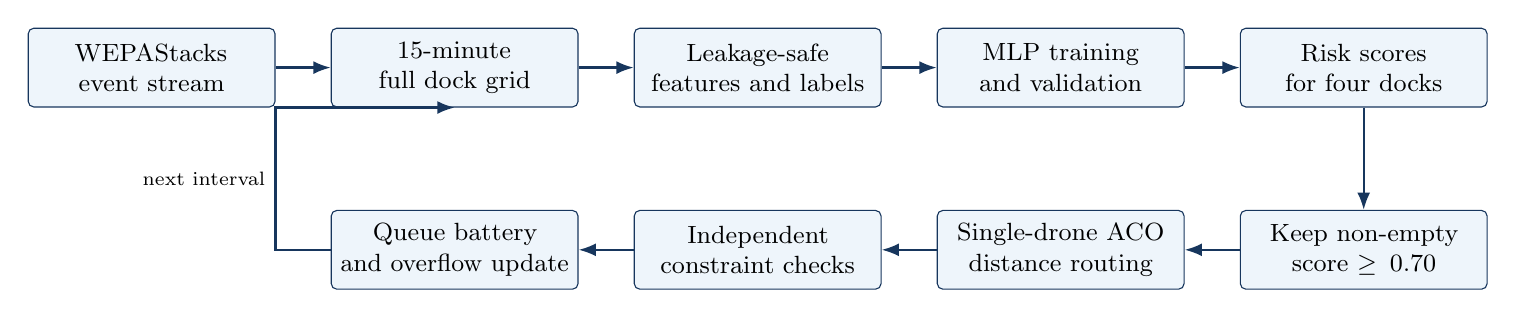
\begin{tikzpicture}[
  node distance=8mm and 7mm,
  box/.style={draw=navy,rounded corners=2pt,fill=paleblue,align=center,minimum height=10mm,text width=29mm,font=\small},
  decision/.style={draw=navy,diamond,aspect=2.2,fill=lightblue,align=center,font=\small,inner sep=1.5pt},
  arrow/.style={-{Latex[length=2.2mm]},thick,draw=navy}
]
\node[box] (events) {WEPAStacks\\event stream};
\node[box,right=of events] (grid) {15-minute\\full dock grid};
\node[box,right=of grid] (features) {Leakage-safe\\features and labels};
\node[box,right=of features] (mlp) {MLP training\\and validation};
\node[box,right=of mlp] (risk) {Risk scores\\for four docks};
\node[box,below=13mm of risk] (active) {Keep non-empty\\score $\geq0.70$};
\node[box,left=of active] (aco) {Single-drone ACO\\distance routing};
\node[box,left=of aco] (validate) {Independent\\constraint checks};
\node[box,left=of validate] (update) {Queue battery\\and overflow update};
\draw[arrow] (events) -- (grid);
\draw[arrow] (grid) -- (features);
\draw[arrow] (features) -- (mlp);
\draw[arrow] (mlp) -- (risk);
\draw[arrow] (risk) -- (active);
\draw[arrow] (active) -- (aco);
\draw[arrow] (aco) -- (validate);
\draw[arrow] (validate) -- (update);
\draw[arrow] (update.west) -| ++(-7mm,0) |- node[pos=0.25,left,font=\scriptsize]{next interval} (grid.south);
\end{tikzpicture}
\caption{Updated data and decision flow. The MLP filters warehouses; its score is not used inside ACO.}
\label{fig:pipeline}
\end{figure}

\subsection{MLP architecture}

The network has two hidden layers. The first maps seven inputs to 32 ReLU units, and the second maps 32 values to 16 ReLU units. A single sigmoid output produces a risk score. Glorot uniform initialisation is used for the dense-layer weights, and all biases start at zero. No dropout layer is used in the drone-compatible implementation.

\begin{figure}[H]
\centering
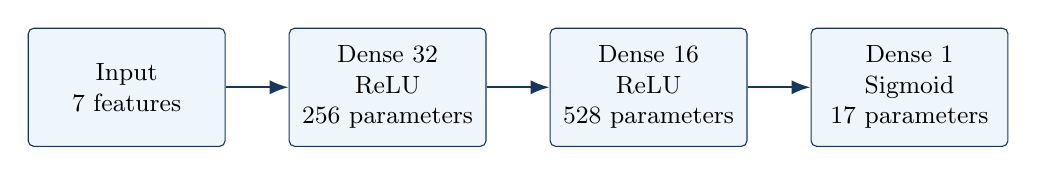
\begin{tikzpicture}[
  layer/.style={draw=navy,rounded corners=2pt,fill=paleblue,minimum width=25mm,minimum height=15mm,align=center,font=\small},
  arrow/.style={-{Latex[length=2.4mm]},thick,draw=navy},
  node distance=8mm
]
\node[layer] (input) {Input\\7 features};
\node[layer,right=of input] (dense1) {Dense 32\\ReLU\\256 parameters};
\node[layer,right=of dense1] (dense2) {Dense 16\\ReLU\\528 parameters};
\node[layer,right=of dense2] (output) {Dense 1\\Sigmoid\\17 parameters};
\draw[arrow] (input) -- (dense1);
\draw[arrow] (dense1) -- (dense2);
\draw[arrow] (dense2) -- (output);
\end{tikzpicture}
\caption{MLP architecture with 801 trainable parameters.}
\label{fig:architecture}
\end{figure}

The forward pass can be written as
\begin{align}
\mathbf{h}_1 &= \operatorname{ReLU}(\mathbf{W}_1\mathbf{x}+\mathbf{b}_1),\\
\mathbf{h}_2 &= \operatorname{ReLU}(\mathbf{W}_2\mathbf{h}_1+\mathbf{b}_2),\\
\hat{p} &= \sigma(\mathbf{w}_3^\top\mathbf{h}_2+b_3).
\end{align}

This structure is relatively small and permits nonlinear interactions. ReLU is selected to reduce the saturation concerns associated with sigmoid hidden units, while a sigmoid output is conventional for binary classification. These architectural motivations follow standard feed-forward neural-network practice \cite{rumelhart1986,glorot2010}; they do not by themselves establish that the architecture is suitable for this dataset.

\subsection{Loss, optimiser, and class imbalance}

The network minimises weighted binary cross-entropy:
\begin{equation}
\mathcal{L}_{\mathrm{BCE}}=-\frac{1}{N}\sum_{n=1}^{N}w_{y_n}
\left[y_n\log \hat{p}_n+(1-y_n)\log(1-\hat{p}_n)\right].
\label{eq:bce}
\end{equation}
Balanced weights computed from the 22,628 training labels are $w_0=0.6925$ and $w_1=1.7984$. They compensate for the 27.80\% positive training rate in the loss, but do not correct unequal temporal coverage across warehouses. Adam is configured with learning rate $10^{-3}$, $\beta_1=0.9$, $\beta_2=0.999$, and $\epsilon=10^{-7}$ \cite{kingma2015}. Training uses mini-batches of 256, at most 100 epochs, and early stopping on validation loss with patience eight and restoration of the best weights.

\subsection{MLP filter and single-drone ACO}

At interval $t$, available goods are $A_{i,t}=Q_{i,t}+a_{i,t}$. For MLP--ACO, the active set is
\begin{equation}
\mathcal{S}_t=\{i\mid A_{i,t}>0\ \land\ \hat p_{i,t}\geq0.70\}.
\label{eq:active-filter}
\end{equation}
Warehouses outside $\mathcal{S}_t$ are absent from the ACO input and cannot appear in its route. For nearest-first, fullest-first, and ACO-current, the active set instead uses the current-fill rule $A_{i,t}/K_i\geq0.80$. This is the only difference between ACO-current and MLP--ACO; both use the same route optimiser.

Each ant begins at depot 0 and maintains the travelled distance. A candidate warehouse $j$ is feasible only if the route can visit it and still return to the depot:
\begin{align}
D_{\mathrm{proj}} &= D_{\mathrm{so\ far}}+d_{ij}+d_{j0},\\
D_{\mathrm{proj}} &\leq D_{\max},\\
D_{\mathrm{proj}}e &\leq B_{\mathrm{available}},
\end{align}
where $e$ is energy per kilometre. Among feasible unvisited warehouses, the transition probability is
\begin{equation}
P(i\rightarrow j)=
\frac{\tau_{ij}^{\alpha}\left(1/(\varepsilon+d_{ij})\right)^{\beta}}
{\sum_{k\in\mathcal{F}}\tau_{ik}^{\alpha}\left(1/(\varepsilon+d_{ik})\right)^{\beta}}.
\label{eq:aco-transition}
\end{equation}
The MLP score and amount of goods do not appear in this transition rule. The implementation uses $\alpha=1$, $\beta=2$, 30 ants, at most 100 iterations, evaporation 0.10, and a 20-iteration stall limit.

For route $R$, the objective is
\begin{equation}
J(R)=1000\,|\mathcal{S}_t\setminus V(R)|+D(R),
\label{eq:aco-objective}
\end{equation}
where $V(R)$ is the set of visited active warehouses. Since every feasible route is limited to 30~km, the penalty makes an additional active visit more important than any possible distance saving. Among routes visiting the same number of active warehouses, the shorter route wins. After each iteration, pheromone evaporates and the global-best route receives an increment proportional to $1/(1+J)$.

After route construction, the 30-unit payload is divided in proportion to available goods at visited warehouses. If $C=\min(30,\sum_{j\in V(R)}A_{j,t})$, then
\begin{equation}
x_{i,t}=C\frac{A_{i,t}}{\sum_{j\in V(R)}A_{j,t}},\qquad i\in V(R).
\end{equation}
The validator recomputes depot endpoints, repeated and filtered nodes, total distance, route energy, payload, and per-warehouse pickup. Goods not collected remain in the queue. Battery is logged after the route and restored before the next interval.

\subsection{Theory-to-code mapping}

\begin{table}[H]
\centering
\caption{Mapping from computational concepts to intended implementation behaviour}
\label{tab:theory-code}
\small
\begin{tabularx}{\textwidth}{p{0.20\textwidth}Yp{0.30\textwidth}}
\toprule
Component & Intended behaviour & Main source file \\
\midrule
Interval grid & Aggregates events and inserts zero-arrival rows for every dock and time bin & \code{src/data_pipeline.py} \\
Historical state & Runs a fixed fullest-first policy intended to exclude future arrivals & \code{src/queue_simulator.py} \\
Features and labels & Builds seven features, future no-drone labels, boundary gaps, and chronological splits & \code{src/feature_builder.py} \\
MLP training & Fits the scaler, class weights, MLP, and early stopping; saves fixed-threshold reports and a validation-threshold diagnostic & \code{src/train_mlp_aco.py} \\
Risk inference & Applies the saved feature order and returns per-warehouse risk scores & \code{src/predict_risk.py} \\
Filtering and pickup & Applies the 0.70 filter, checks route limits, allocates payload proportionally, and evaluates Eq.~\eqref{eq:aco-objective} & \code{src/routing_utils.py} \\
ACO primary method & Constructs a candidate single-drone route using Eq.~\eqref{eq:aco-transition} and updates pheromone & \code{src/aco_optimizer.py} \\
Greedy baselines & Implements nearest-first and fullest-first policies & \code{src/baselines.py} \\
Validation & Recomputes payload, battery, visited-pickup, and demand checks separately from route construction & \code{src/solution_validator.py} \\
Rolling simulation & Updates queues, battery, overflow, and route logs over time & \code{src/rolling_simulation.py} \\
\bottomrule
\end{tabularx}
\end{table}

\section{Experimental Method}

\subsection{Reproducibility settings}

The current experiment configuration specifies seed 42 for Python, NumPy, and TensorFlow. Deterministic TensorFlow operations are requested where supported. The recorded development environment lists Python 3.9.6, TensorFlow 2.20.0, Keras 3.10.0, NumPy 2.0.2, pandas 2.3.3, and scikit-learn 1.6.1. These details should be captured again for the final run, and exact bitwise equality across hardware and library versions should not be assumed.

\begin{table}[H]
\centering
\caption{Main MLP hyperparameters}
\label{tab:hyperparameters}
\small
\begin{tabular}{ll@{\qquad}ll}
\toprule
Parameter & Value & Parameter & Value \\
\midrule
Interval & 15 minutes & Horizon & 4 intervals \\
Capacities & 200, 80, 80, 80 & Congestion level & 80\% of capacity \\
Hidden units & 32, 16 & Trainable parameters & 801 \\
Learning rate & 0.001 & Batch size & 256 \\
Maximum epochs & 100 & Early-stopping patience & 8 \\
Training boundary & Day 60 & Validation boundary & Day 74 \\
Operational threshold & Fixed at 0.70 & Validation diagnostic & 0.9313 \\
\bottomrule
\end{tabular}
\end{table}

\subsection{Evaluation metrics}

Accuracy alone is insufficient when class balance and temporal coverage differ across docks. Precision measures how many warnings are correct. Recall measures how many threshold cases are detected. F1 balances precision and recall. Balanced accuracy averages sensitivity and specificity. Average precision summarises the precision--recall curve \cite{saito2015}. The confusion matrix and per-dock support are essential because strong global performance can still reflect a dock-identity shortcut rather than general temporal prediction.

For routing, the metrics are overflow, collected goods, energy, distance, number of sorties, active-warehouse visit rate, runtime, and independently recomputed constraint violations. The primary comparison is MLP--ACO against nearest-first, fullest-first, and ACO-current. A complete routing result requires the entire held-out period and repeated ACO seeds. The present operational run does not meet that requirement and is labelled as a smoke test.

\section{Results}

\subsection{Training behaviour}

Training stopped after 75 epochs. The lowest recorded validation loss was 0.04998 at epoch 67 using one-based numbering; early stopping then restored those weights. Figure~\ref{fig:training-results} shows rapid improvement during the first epochs and a much slower change afterwards. Similar training and validation curves are useful evidence against severe overfitting in this run, but they do not address the warehouse-coverage shift discussed below.

\begin{figure}[H]
\centering
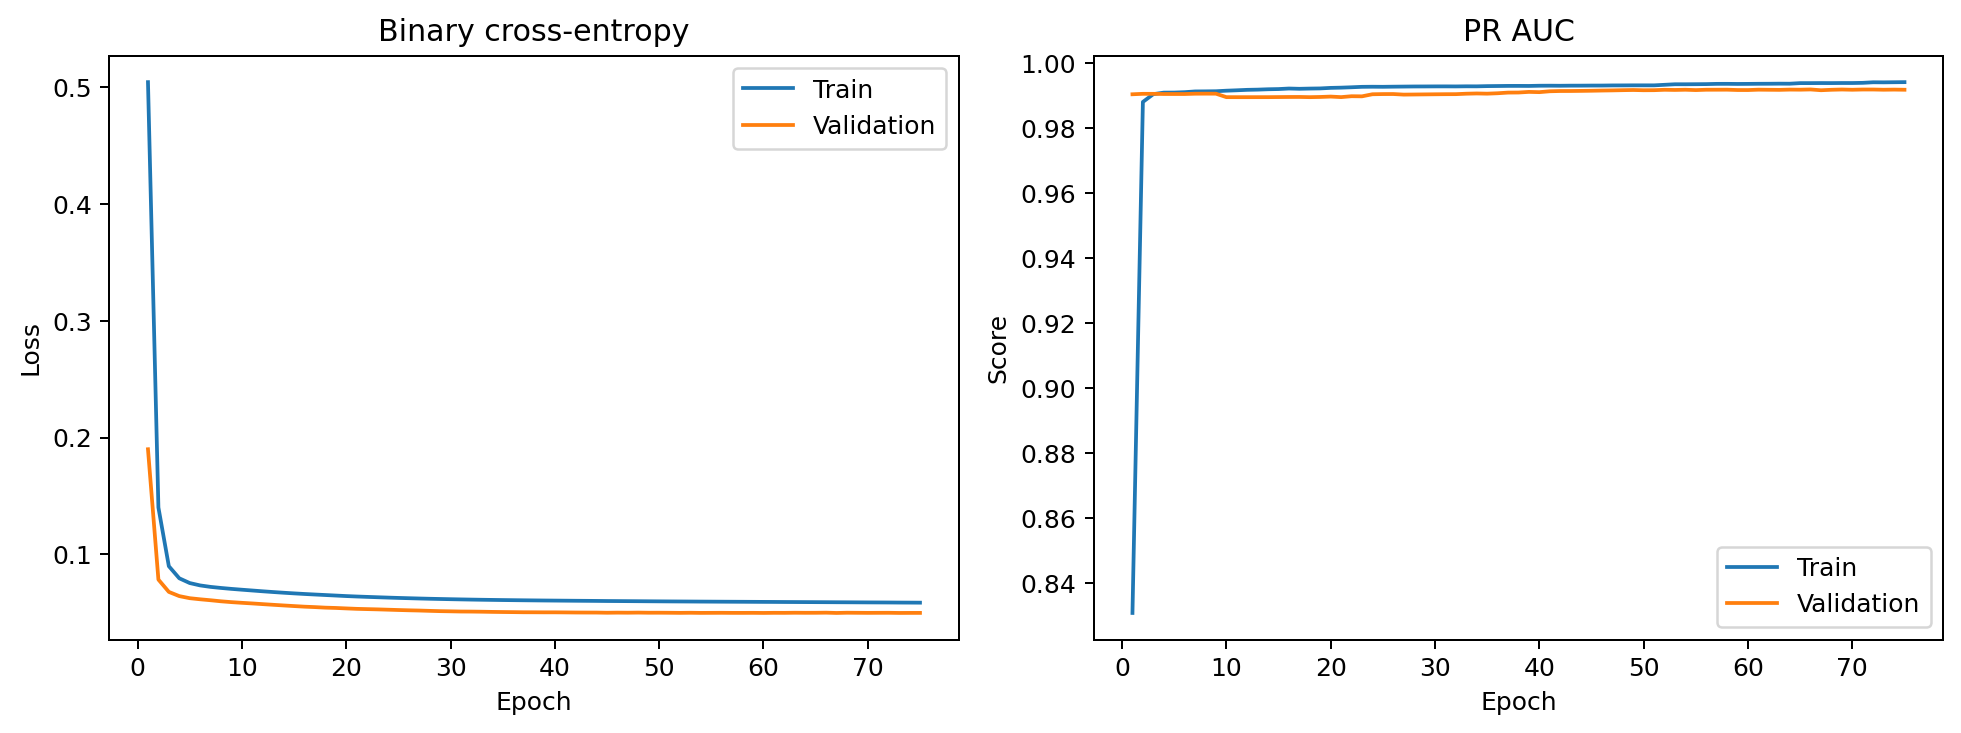
\includegraphics[width=0.96\textwidth]{training_history.png}
\caption{Recorded training and validation binary cross-entropy and PR--AUC.}
\label{fig:training-results}
\end{figure}

\subsection{Held-out prediction results}

Table~\ref{tab:prediction-baselines} evaluates the fixed operational threshold of 0.70 on the chronological test set. The always-negative rule illustrates why accuracy alone is insufficient: it obtains 80.13\% accuracy while detecting no positive case. The current-fill rule is stronger, but the MLP increases recall from 78.07\% to 95.45\% while retaining 98.59\% precision. The MLP therefore exceeds both declared prediction baselines on this test set.

\begin{table}[H]
\centering
\caption{Prediction comparison on 5,532 chronological test samples}
\label{tab:prediction-baselines}
\small
\begin{tabular}{lrrrrr}
\toprule
Method & Accuracy & Balanced accuracy & Precision & Recall & F1 \\
\midrule
Always negative & 80.13\% & 50.00\% & 0.00\% & 0.00\% & 0.00\% \\
Current fill $\geq0.80$ & 95.64\% & 89.04\% & 100.00\% & 78.07\% & 87.69\% \\
\rowcolor{paleblue}MLP score $\geq0.70$ & 98.83\% & 97.56\% & 98.59\% & 95.45\% & 96.99\% \\
\bottomrule
\end{tabular}
\end{table}

The MLP test PR--AUC is 99.38\% and ROC--AUC is 99.84\%. At the fixed threshold, the confusion matrix contains 4,418 true negatives, 15 false positives, 50 false negatives, and 1,049 true positives. A false negative is operationally important because the hard filter removes that warehouse from ACO; a false positive can instead create an unnecessary active candidate.

\begin{figure}[H]
\centering
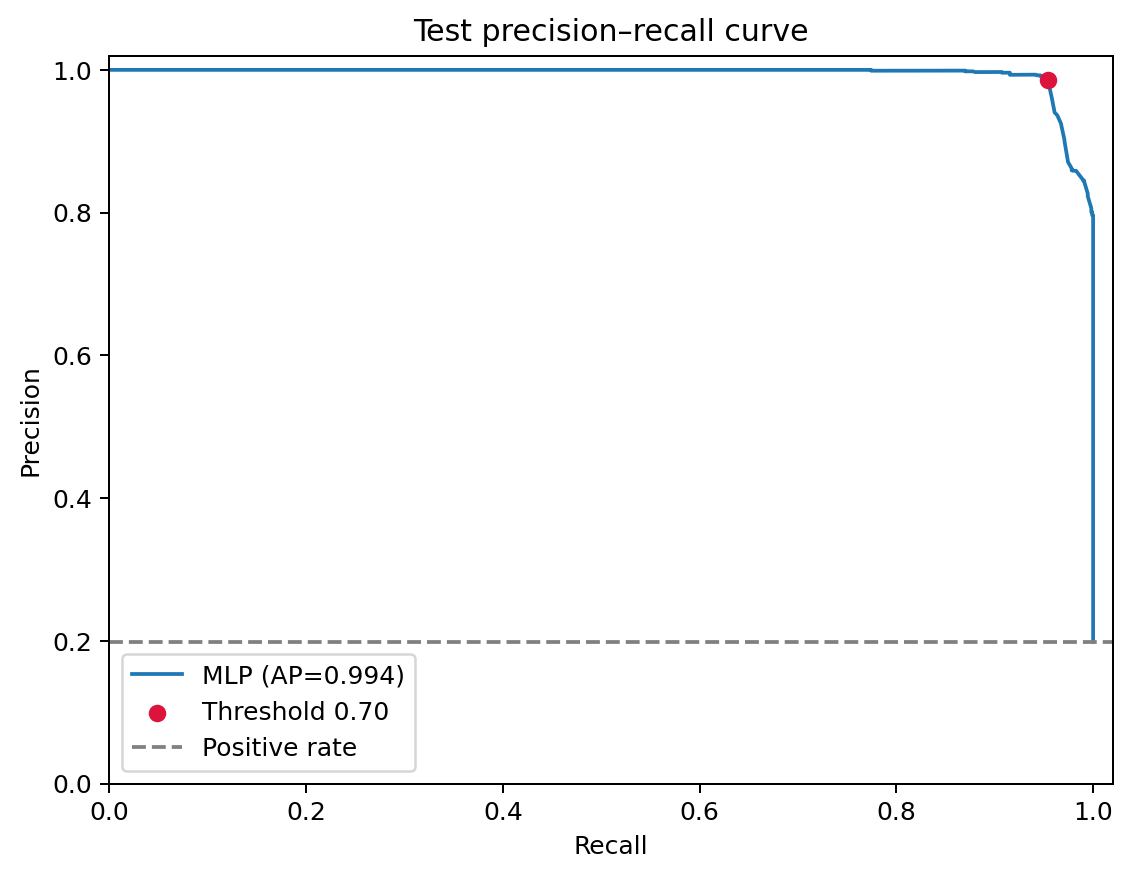
\includegraphics[width=0.62\textwidth]{precision_recall_curve.png}
\caption{Test precision--recall curve. The red point is the fixed operational threshold of 0.70; the dashed line is the test positive rate.}
\label{fig:pr-curve}
\end{figure}

\subsection{Warehouse support and interpretation}

The global result does not provide equal evidence for all warehouses. Warehouse~1 contains both classes and all 1,099 positive test samples. Warehouses~2--4 contain no positive test samples, so their positive-class precision, recall, F1, and AUC are not interpretable.

\begin{table}[H]
\centering
\caption{Test support and interpretable MLP metrics by warehouse}
\label{tab:warehouse-support}
\small
\begin{tabular}{lrrrrr}
\toprule
Warehouse & Samples & Positive & Negative & Recall & F1 \\
\midrule
1 & 1,383 & 1,099 & 284 & 95.45\% & 96.99\% \\
2 & 1,383 & 0 & 1,383 & Not defined & Not defined \\
3 & 1,383 & 0 & 1,383 & Not defined & Not defined \\
4 & 1,383 & 0 & 1,383 & Not defined & Not defined \\
\bottomrule
\end{tabular}
\end{table}

This support pattern prevents a claim that the model detects positive congestion cases at Warehouses~2--4. Nevertheless, Warehouse~1 itself contains 284 negative and 1,099 positive cases, so its result is not based only on warehouse identity. An ablation without the one-hot warehouse features is still required to quantify their contribution.

\subsection{Routing smoke test}

The current operational artifact covers 20 test intervals, 80 warehouse rows, and one ACO seed. It is not a full held-out or repeated-seed experiment. Table~\ref{tab:routing-smoke} is included to verify the updated single-drone flow and to expose its trade-off, not to establish superiority.

\begin{table}[H]
\centering
\caption{Preliminary 20-interval, one-seed routing smoke test}
\label{tab:routing-smoke}
\small
\begin{tabular}{lrrrrrr}
\toprule
Policy & Overflow & Collected & Distance & Energy & Sorties & Violations \\
\midrule
Nearest-first & 97 & 480 & 160 & 160 & 16 & 0 \\
Fullest-first & 97 & 480 & 160 & 160 & 16 & 0 \\
ACO-current & 97 & 480 & 160 & 160 & 16 & 0 \\
\rowcolor{paleblue}MLP--ACO & 0 & 600 & 200 & 200 & 20 & 0 \\
\bottomrule
\end{tabular}
\end{table}

In this short run, MLP--ACO activates and serves a route in all 20 intervals, whereas the current-fill policies do so in 16. The additional four sorties coincide with 120 more collected units and 97 fewer overflow units, but also with 40 additional distance and energy units. Because the run contains one seed and a small prefix of the test stream, these differences may depend on the selected interval window and cannot answer the research question.

\subsection{Implementation verification}

A fresh run of the current test suite completed 21 tests with no failures. The tests exercise the 0.70 inclusion boundary, exclusion of empty and filtered warehouses, depot endpoints, repeated-node rejection, payload and demand limits, energy and explicit distance limits, fixed-seed behaviour, per-interval battery reset, queue updates, and a small exact-reference comparison. This is evidence for those cases only; it is not a proof that every state or route is correct.

\section{Discussion}

\subsection{Answer to the research question}

The prediction evidence is positive but narrow. At the fixed 0.70 threshold, the MLP improves F1 and recall over the current-fill rule on the present chronological test set. This supports the claim that the seven features contain information beyond the instantaneous 0.80 fill decision for Warehouse~1. It does not establish positive-case performance for Warehouses~2--4, which have no positive validation or test support.

The operational part of the research question remains open. The smoke test is consistent with the idea that earlier MLP activation can exchange extra trips and energy for lower overflow. However, 20 intervals and one seed are insufficient to estimate performance over the full test period or stochastic variation. No final claim that MLP filtering improves ACO is made.

\subsection{Training loss versus the practical objective}

Weighted binary cross-entropy rewards agreement between the sigmoid score and the simulated binary label. The practical objective concerns overflow, collected goods, travel, energy, and missed service. The two objectives are related but not identical. Reducing BCE may move a score without changing which side of 0.70 it occupies, producing no routing change. Conversely, a small score change across 0.70 changes the ACO candidate set discontinuously.

The ACO objective also differs from the operational objective. Equation~\eqref{eq:aco-objective} maximises the number of active warehouses visited before minimising distance. It does not directly reward collected quantity or avoided overflow. For example, it can prefer visiting two small active warehouses over one high-volume warehouse when distance prevents visiting all three. Proportional pickup allocation is applied only after the route is chosen. These mismatches are tolerated to keep the algorithm transparent, but they must be monitored through overflow, collection, distance, and energy rather than through BCE or ACO objective value alone.

\subsection{Implications}

The fixed operational threshold is 0.70, whereas the validation-F1 diagnostic threshold is 0.9313. The lower operational threshold is expected to admit more warehouses and favour recall, but its value was specified rather than selected by an operational validation study. A threshold-sensitivity experiment is therefore necessary. The sigmoid value should be called a risk score until calibration has been demonstrated.

The single-drone design makes the algorithm easier to explain and validate. It also reduces the combinatorial difficulty: with at most four active warehouses there are only 24 complete visit orders before considering subsets. ACO remains a valid stochastic routing study, but an exact enumerator is computationally practical for this experiment and should be used more extensively as a reference.

\subsection{Limitations}

\begin{enumerate}
  \item \textbf{Simulated target.} Queue length and congestion are generated from assumed capacities, drone behaviour, and a no-drone future scenario. The model predicts this construction, not measured warehouse congestion.
  \item \textbf{Current-state contribution to the label.} The target starts from current available goods, so some positive cases are already at the 80\% boundary. The task combines current-state detection with future forecasting.
  \item \textbf{Warehouse coverage shift.} Warehouses~2--4 end early in the supplied event stream and have no positive validation or test labels.
  \item \textbf{Ambiguous zero intervals.} Missing or inactive coverage is encoded in the same way as an active dock with zero arrivals.
  \item \textbf{Dominant Dock 1.} Dock~1 contains 93.26\% of inbound events, so the fitted shared model may be strongly influenced by its operating pattern.
  \item \textbf{Potential warehouse shortcut.} One-hot identity features may exploit the unequal support pattern; their effect has not yet been measured by ablation.
  \item \textbf{Uncalibrated score.} Weighted BCE can produce useful ranking without a calibrated probability, and no reliability analysis is currently reported.
  \item \textbf{Limited feature set.} The baseline excludes hour-of-day, shift, robot state, downtime, service completions, and SKU mixture.
  \item \textbf{Simplified single-drone physics.} Battery is restored every 15 minutes and the model omits flight duration, charging time, weather, no-fly zones, and collision avoidance.
  \item \textbf{Hard filtering.} A score change from 0.699 to 0.700 can change routing eligibility even though the underlying states are almost identical.
  \item \textbf{Objective mismatch.} ACO minimises unvisited active warehouses and distance, not expected overflow or collected quantity.
  \item \textbf{Incomplete routing evaluation.} The reported operational comparison contains 20 intervals and one ACO seed; it cannot estimate full-period or repeated-seed behaviour.
  \item \textbf{Small routing instance.} With four warehouses, exact enumeration may be more appropriate than ACO unless the study is explicitly framed as a prototype for larger instances.
\end{enumerate}

\section{Recommended Refinements}

One important improvement is to obtain data that distinguish an active dock with no arrivals from an inactive or unobserved dock. A \texttt{dock\_active} field, operating calendar, and documented reason for the early termination of Warehouses~2--4 would support a more defensible temporal grid. Real queue length, service completions, incident logs, and confirmed capacities could then be used to assess Eq.~\eqref{eq:target} against an observed target.

Model evaluation should preserve chronological splits and report support for every metric. The first ablation should remove warehouse one-hot inputs; a second should evaluate only cases whose current fill is below 0.80, thereby isolating genuine congestion onset. Probability calibration should be assessed with a reliability diagram and Brier score. Any changes made after inspecting the current test results require a new untouched test period.

The 0.70 routing threshold should be varied on validation simulations, for example alongside 0.50 and 0.90, and compared using overflow--energy trade-offs. Candidate policies should also test a minimum pickup load. A decision-aware extension could replace the count-based penalty with estimated overflow cost, although this would make the algorithm more complex.

The final routing experiment should run nearest-first, fullest-first, ACO-current, and MLP--ACO on identical copies of the complete held-out stream. ACO should use all ten configured seeds. Results should include mean, standard deviation, and confidence intervals for overflow, goods collected, energy, distance, active visits, sorties, and runtime. Because there are at most four warehouses, every active set can also be compared with the exact reference solver to quantify any ACO optimality gap.

\section{Conclusion}

The updated system has a clear two-stage interface: the MLP produces four risk scores, a fixed 0.70 filter selects non-empty warehouses, and single-drone ACO builds a distance-based route over only those warehouses. The ACO objective penalises unvisited active warehouses before distance, and payload is divided proportionally after route construction. This description matches the current configuration and implementation; earlier multi-drone, urgency-weighted, and daily-battery formulations are not part of the reported method.

On the current chronological test set, the MLP exceeds the always-negative and current-fill prediction baselines, reaching 96.99\% F1 at the fixed threshold. The result is supported for Warehouse~1 but not for positive cases at Warehouses~2--4. The routing smoke test shows a favourable overflow--energy trade-off for MLP--ACO over 20 intervals, but its scope is too small for a final operational conclusion. The complete held-out, ten-seed experiment remains necessary before claiming that MLP filtering improves routing.

\section*{Reproducibility Checklist}
\addcontentsline{toc}{section}{Reproducibility Checklist}

\begin{itemize}
  \item Dataset file: \code{wepastacks_inbound_clean.csv}.
  \item Single-drone MLP artifacts: \code{model_outputs_single_drone/mlp_congestion_aco.keras}, \code{feature_scaler.pkl}, \code{model_configuration.json}, \code{training_history.csv}, \code{metrics.json}, and \code{test_predictions.csv}.
  \item Prediction tables and figures: \code{model_outputs_single_drone/prediction_baseline_comparison.csv}, \code{per_warehouse_classification_metrics.csv}, and the \code{figures} directory.
  \item Command-line training entry point: \code{run_training.py}.
  \item Integrated experiment configuration: \code{config/experiment.yaml}.
  \item Routing entry point: \code{run_experiment.py}.
  \item Test command: \code{PYTHONPYCACHEPREFIX=/tmp/assignment2_pycache .venv/bin/python -m unittest discover -s tests -v}.
  \item Current verification: 21 tests passed in the available virtual environment; rerun immediately before submission.
  \item Preliminary operational outputs: \code{outputs_single_drone}; \code{experiment_scope.json} records that the present run is not the full test period.
  \item Required final evidence: complete held-out routing runs and ten seeds for each stochastic ACO policy.
\end{itemize}

\appendix
\section{Configured Drone Experiment}

\begin{table}[H]
\centering
\caption{Simulated warehouse coordinates and capacities}
\small
\begin{tabular}{lrrr}
\toprule
Node & $x$ (km) & $y$ (km) & Capacity (cargo units) \\
\midrule
Central depot 0 & 0 & 0 & Not applicable \\
Warehouse 1 & 3 & 4 & 200 \\
Warehouse 2 & -5 & 2 & 80 \\
Warehouse 3 & 6 & -3 & 80 \\
Warehouse 4 & -4 & -6 & 80 \\
\bottomrule
\end{tabular}
\end{table}

\begin{table}[H]
\centering
\caption{Configured single simulated drone}
\small
\begin{tabular}{lrrrr}
\toprule
Drone & Payload & Battery & Energy/km & Maximum route \\
\midrule
1 & 30 & 30.0 & 1.0 & 30 km \\
\bottomrule
\end{tabular}
\end{table}

Battery is reset before every 15-minute interval. This represents replacement or charging at the depot and is not an optimised charging schedule. The values in this appendix are experimental assumptions and must not be attributed to the WEPAStacks warehouse.

\section{Metric Definitions}

For true positives $TP$, false positives $FP$, true negatives $TN$, and false negatives $FN$:
\begin{align}
\mathrm{Precision} &= \frac{TP}{TP+FP}, &
\mathrm{Recall} &= \frac{TP}{TP+FN},\\
\mathrm{Specificity} &= \frac{TN}{TN+FP}, &
\mathrm{F1} &= \frac{2\,\mathrm{Precision}\,\mathrm{Recall}}
{\mathrm{Precision}+\mathrm{Recall}},\\
\mathrm{Balanced\ Accuracy} &= \frac{\mathrm{Recall}+\mathrm{Specificity}}{2}.
\end{align}
The Brier score is the mean squared difference between a predicted score and the binary target. It is not reported in the current artifact set. A Brier score and reliability plot are required before the sigmoid output can be interpreted as a calibrated probability.

\begin{thebibliography}{9}

\bibitem{rumelhart1986}
D. E. Rumelhart, G. E. Hinton, and R. J. Williams.
Learning representations by back-propagating errors.
\emph{Nature}, 323:533--536, 1986.

\bibitem{glorot2010}
X. Glorot and Y. Bengio.
Understanding the difficulty of training deep feedforward neural networks.
In \emph{Proceedings of AISTATS}, pages 249--256, 2010.

\bibitem{kingma2015}
D. P. Kingma and J. Ba.
Adam: A method for stochastic optimization.
In \emph{International Conference on Learning Representations}, 2015.

\bibitem{dorigo1997}
M. Dorigo and L. M. Gambardella.
Ant colony system: A cooperative learning approach to the traveling salesman problem.
\emph{IEEE Transactions on Evolutionary Computation}, 1(1):53--66, 1997.

\bibitem{saito2015}
T. Saito and M. Rehmsmeier.
The precision-recall plot is more informative than the ROC plot when evaluating binary classifiers on imbalanced datasets.
\emph{PLOS ONE}, 10(3):e0118432, 2015.

\bibitem{projectdocs}
WEPAStacks project documentation.
\emph{Dataset Analysis Report, MLP Training Specification, MLP Training Report, Single-Drone MLP--ACO Implementation Guide, and Assessment Criteria}.
Internal assignment documents, 2026.

\end{thebibliography}

\end{document}
